\subsection{Ejercicio 2}
	En el ejercicio 2 se pedía crear e inicializar dos directorios y tablas de páginas según los mapas de memoria dados en el enunciado. Los 
directorios de página fueron definidos como \verb=page_dir_pintor= y \verb=page_dir_kernel= en el archivo \verb=kernel.asm=. Los archivos 
\verb=kernel-traductor_paging.asm= y \verb=pintor_paging.asm= contienen las tablas ya inicializadas. 

	Para empezar a usar la paginación, se debe habilitar en el registro \code{cr0}, pero antes hay que inicializar los directorios y tablas de paginas 
necesarias. 

	Para inicializar los directorios se definió la subrutina \verb=page_init= que define la primera entrada de ambos directorios con su primer tabla 
(\verb=page_table_0= para el directorio del \keyword{kernel} y \verb=page_table_0_pintor= para el directorio del pintor). Antes de ser llamada, hay que 
especificar un valor válido para el esp, que controla el \keyword{stack} principal, ya que al hacer el \code{call} a la función \verb=page_init=, el 
programa debe conocer la dirección a la cual regresar para continuar la ejecución. 

Ya dentro de la subrutina, se les agregan los \keyword{flags} de \code{supervisor}, \code{read/write} y \code{present} a las primeras entradas de cada 
directorio, junto con la dirección correspondiente a su primer tabla. 
La estructura de un descriptor de directorio de página es el siguiente:

\begin{center}
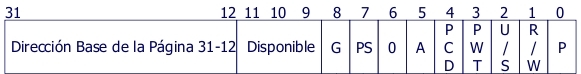
\includegraphics[scale=0.5]{descriptorpagina.jpg}
\end{center}

\begin{itemize}
	\item\code{Dirección}: se toman los \keyword{bits} 31 al 12 inclusive (20 \keyword{bits}) de la dirección de memoria recibida por el módulo 
de segmentación (dirección lineal) y esto servirá para localizar la tabla de página correspondiente.
	\item\code{Bit PS}: es el \keyword{bit} 7 y determina el tamaño de la pagina, que puede ser de 4Kb o 4Mb, pero para esto último se necesita que 
el modo \code{PSE} de paginación extendida esté activado (no requerido en el trabajo actual).
	\item\code{Bit A}: \code{Accessed}, determina si se escribió o leyó de una página o no. Es el \keyword{bit} 5.
	\item\code{Bit PCD}: este \keyword{bit} deshabilita el caché, por lo que permanecerá en 0. Es el \keyword{bit} 4.
	\item\code{Bit PWT}: es para habilitar el modo \code{Write-through} de la \keyword{caché}, no lo utilizamos.
	\item\code{Bit U}: determina el nivel de privilegio, si no esta \keyword{seteado}, el privilegio es de \code{Supervisor} (el mas alto). 
	\item\code{Bit R/W}: habilita la lectura y escritura en las páginas, lo requerimos en el trabajo.
	\item\code{Bit P}: dice si la pagina esta presente en la memoria. Lo habilitamos para no producir una \code{Page Fault}.
\end{itemize}
	
\subsubsection{Tablas de página} 
	Como se dijo anteriormente, las tablas de página estan definidas en los archivos \verb=kernel-traductor_paging.asm= y \verb=pintor_paging.asm=. Cada 
tabla de páginas tiene un mapeo de memoria diferente, el cual fue definido a mano usando \keyword{macros} para ayudar. En cada tabla se tuvo que hacer 
\keyword{identity mapping} para algunas direcciones, otras fueron mapeadas a lugares de memoria fijos (como en el caso de la memoria de video) y otras no 
fueron especificadas, esto es, inicializarlas en 0.

	Para realizar el mapeo de memoria se utilizaron \keyword{macros} que permitieron definir las entradas de la tabla correspondientes fácilmente. A 
continuación un ejemplo de la macro utilizada para \keyword{identity mapping}:

\begin{verbatim}
	%assign i 0x0000 
	%rep    0x009 
	    dd 	i | 3 
	%assign i i+4096 
	%endrep 
\end{verbatim}

	Primero se asigna \code{i} a la dirección sobre la que se quiere hacer \keyword{identity mapping}, después se hace un \code{or} con el valor 3, que 
al igual que en los descriptores de directorios, esto quiere decir que la página tendrá privilegios de supervisor, estará presente y será de lectura/escritura, 
luego se repite $n$ veces con $n$ la cantidad de paginas a \keyword{mapear}.

    Las direcciones que tenían que ser mapeadas a una página específica fueron definidas individualmente, por ejemplo: 

\begin{verbatim}
		%assign i 0x13000 
		%rep 0x001 

			dd 0xb8000 | 3 

		%assign i i+4096 
		%endrep 
\end{verbatim}

	La diferencia con el código anterior, es que éste tiene especificada la dirección a la cual \keyword{mapear}, en vez de usar al variable \code{i}. 

    	Finalmente las direcciones que no se debían asignar, fueron dejadas en 0. Esto significa que ni siquiera estarán presentes en memoria, ni podrán 
ser utilizadas. Dejamos, por legibilidad, lineas como \verb=%rep 0x0001= o \verb=dd 0 | 0=. Luego en el \keyword{kernel} se completan ambas tablas de página con 0. 

	Para poder hacer un \code{call} a \verb=page_init= en el \keyword{kernel} se definió antes el valor de la pila de \keyword{kernel} en \code{0x7FFC}
(\code{esp} y \code{ebp}). Después de tener inicializados los directorios se copia la dirección del directorio de páginas de \keyword{kernel} al \code{cr3} 
y se habilita la paginación poniendo en 1 el \keyword{bit} más significativo del \code{cr0}. 

    En la segunda parte del ejercicio, pide escribir el nombre del grupo en la esquina superior izquierda. Para ello, se accede a la memoria de video a 
través de su respectivo segmento definido en la \code{GDT}, y se usa un código similar al usado en el ejercicio 1 para limpiar la pantalla, con la 
diferencia que está la instrucción \code{lodsb} la cual lee un \keyword{byte} de la dirección \code{ds:esi} y lo guarda en el registro \code{al}. Previamente 
el registro \code{esi} fue apuntado a la dirección a donde se encuentra el mensaje a escribir. Usando otra vez la instrucción \code{stosw} se escribe el 
mensaje en pantalla.

